\documentclass{beamer}
\usepackage{booktabs}
\usepackage{tabu}
\usepackage{tikz}
\usepackage{pgfplots}
\usepackage[letterspace=110]{microtype}
\usepackage[bitstream-charter]{mathdesign}
\usepackage[light]{sourcecodepro}
\usepackage{caption}
\captionsetup[figure]{labelformat=empty}
\usetheme{metropolis}
\setbeamercolor{normal text}{fg=black,bg=white}
\setbeamercolor{title separator}{fg=red,bg=white}
\setbeamerfont{frametitle}{family=\ttfamily\lsstyle,series=\mdseries,size=\Large}
\setbeamerfont{title}{family=\ttfamily\lsstyle,series=\mdseries,size=\huge}

\let\theframetitle\frametitle
\renewcommand\frametitle[1]{\theframetitle{\MakeUppercase{#1}}}

\usepackage[utf8]{inputenc}
\title{\texttt{tell me to survive}}
\author{David Li, Michael Mauer, and Andy Jiang}
\institute{Cornell University}
\date{May 17, 2016}

\begin{document}

\frame{\titlepage}

\begin{frame}
\frametitle{Motivation}

% I'm adding some comments to elucidate what I'm thinking about saying
% for each of these slides

\begin{itemize}
\item<1-> Lots of programming games already
% So we have to teach people how do OOP ("summative"...?)
% paradigm shift is hard
\item<2-> Object-oriented programming?
% The issue is in teaching to think in classes and objects ("formative"...?)
\item<3-> Object-oriented thinking!
% Comparing to the real world is a good way to explain. logical.
\item<4-> Concepts from real world examples
% The trick is to go from concepts to to code, which is concreteness fading
\item<5->\alt<6->{\textbf{Game mechanics} to code?}{Concepts to code?}
\end{itemize}
\end{frame}

% Listing things looked bad for the slides. So I wrote out concepts.
% basic idea is, there's stuff with components of our game in isolation
% but not together.
\begin{frame}
\frametitle{Related Work}
\begin{columns}[onlytextwidth]
  % This is ugly as fuck, sorry
  \begin{column}{.3\textwidth}
    \alt<2->{
      \alt<3->{
        \alt<4->{
        \begin{figure}
          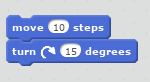
\includegraphics[width=\textwidth]{scratch}\\
          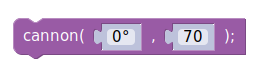
\includegraphics[width=\textwidth]{blocklygames_unfaded}\\
          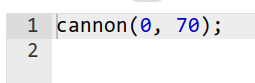
\includegraphics[width=\textwidth]{blocklygames_faded}
        \end{figure}

        }{
          \begin{figure}
            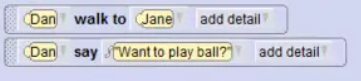
\includegraphics[width=1.2\textwidth]{lookingglass}
            \caption{Looking Glass OOP (credit: Looking Glass tutorial)}
          \end{figure}
        }
      }{
        \begin{figure}
          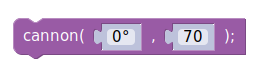
\includegraphics[width=\textwidth]{blocklygames_unfaded}
        \end{figure}
        \begin{figure}
          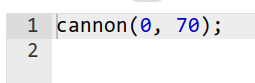
\includegraphics[width=\textwidth]{blocklygames_faded}
          \caption{Blockly Games concreteness fading}
        \end{figure}
      }
    }{
      \begin{figure}
        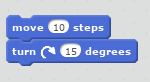
\includegraphics[width=\textwidth]{scratch}
        \caption{Scratch's block interface}
      \end{figure}
    }
  \end{column}
  \begin{column}{.65\textwidth}
    \alt<4->{\textbf{Key inspirations:}}{}
    \begin{itemize}
      % in fact, this is a pretty standard appraoch!
    \item<1-> Visual Programming
      \begin{itemize}
      \item\alt<4->{\textbf{Scratch}}{Scratch}, Looking Glass,
        CodeSpells, \alt<4->{\textbf{Blockly Games}}{Blockly Games},
        \alt<4->{\textbf{LightBot}}{LightBot}, Human Resource Machine,
        …
      \end{itemize}
      % Blockly Games (but not one coherent game)
    \item<2-> Concreteness Fading
      \begin{itemize}
      \item\alt<4->{\textbf{Blockly Games}}{Blockly Games}
      \end{itemize}
    \item<3-> Object-Oriented Programming
      \begin{itemize}
      \item Looking Glass, CodeSpells
      \end{itemize}
    \end{itemize}
    % The \alt things give us a copy of the slide at the end with the
    % relevant things bolded - this highlights our direct inspirations for
    % what we are doing
  \end{column}
\end{columns}
\end{frame}

\begin{frame}
\frametitle{Related Work}
\begin{itemize}[<+->]
\item Combination is key
\end{itemize}
\end{frame}

\begin{frame}
\frametitle{Final Project}
\begin{itemize}[<+->]
% Maybe the concept progression could go here
\item Idea: solve puzzles with object-oriented code
\item Scope: OOP fundamentals
% TODO: ease transition from what to what?
\item Goal: ease transition
\end{itemize}
\end{frame}

\begin{frame}
\frametitle{Final Project}
Force use of OOP via:
\begin{itemize}
% Verbally cover the examples from the write-up
\item Limited block complexity
\item Block limit
\end{itemize}
\end{frame}

% Okay so it's kinda weird to give this it's own slide title
% but I thought putting on to the slide didn't look very good
% besides, despite more bullet points the previous section might
% take more time
\begin{frame}[fragile]
\frametitle{Concreteness Fading}
\begin{columns}[onlytextwidth]
  \begin{column}{.45\textwidth}
    \begin{figure}
      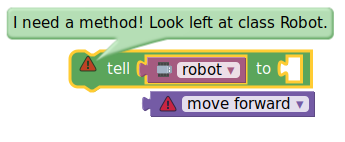
\includegraphics[width=\textwidth]{../report/block_unfaded}
    \end{figure}
    \vspace{-7mm}\centerline{$\Downarrow $}\vspace{-2.5mm}
    \begin{figure}
      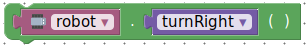
\includegraphics[width=\textwidth]{../report/block_faded}
    \end{figure}
    \vspace{-5mm}\centerline{$\Downarrow $}\vspace{-2.5mm}
\begin{verbatim}
robot.moveForward()
robot.turnRight()
\end{verbatim}
  \end{column}
  \begin{column}{.45\textwidth}
    Three stages:
    \begin{enumerate}
    \item Textual description
    \item Python syntax on blocks
    \item Code editor
    \end{enumerate}
  \end{column}
\end{columns}
\end{frame}

\begin{frame}
\frametitle{Concreteness Fading}
Considerations:
\begin{itemize}
\item<1-> \alt<2>{\textbf{Fading + new concept = confusion}}{Fading + new concept = confusion}
  \begin{itemize}
  \item<2-> Introduce either a new concept or a faded block per level
  \end{itemize}
\item<1-> \alt<3>{\textbf{Scaffolding}}{Scaffolding}
  \begin{itemize}
  \item<3-> Keep object hierarchy, warnings, tooltips after fading
  \item<3-> Unintended: players used faded blocks to help them write code
  \end{itemize}
\end{itemize}
\end{frame}

\begin{frame}
\frametitle{User Study}
\begin{itemize}
\item ``Robot Commander Aptitude Test''
\item 5 questions
\item Mix of syntax and concepts
% Once we have a definite number of results, this might
% be the place to say how many we tested on
% or that can go in results.
\end{itemize}
\end{frame}

\begin{frame}
\frametitle{Results}
\begin{itemize}
\item<1-> 12 people completed the game and post-test
\item<1-> Pre-test mean: 3.167 (s = 1.267)
\item<1-> Post-test mean: 4.25 (s = 0.754)
\item<2-> Statistically significant
    \begin{itemize}
    \item paired t-test
    \item t(11) = 3.767, p $\approx$ 0.003
    \end{itemize}
\end{itemize}
\end{frame}

\begin{frame}
\frametitle{Results}
Individual questions:
\begin{center}
\begin{tabu}{lllll}
\toprule
Question & Concepts & Significant? & $p$ & $\chi^2$ \\
\midrule
1 & Inheritance & No & 0.2482 & 1.333 \\
2 & Instantiation & \textbf{Yes} & 0.0133 & 6.125 \\
3 & Method invocation & No & 0.1336 & 2.250 \\
4 & Overriding & No & 0.4795 & 0.500 \\
5 & Subclassing & No & 0.4795 & 0.500 \\
\bottomrule
\\
\end{tabu}
\end{center}

\end{frame}


\begin{frame}
\frametitle{Results}
Confounding factors:
\begin{itemize}
\item<1-> Learning during the pre-test
\item<2-> Not completed in one session
\end{itemize}
\end{frame}

\begin{frame}
\frametitle{Results}
\begin{columns}[onlytextwidth]
  \begin{column}{.5\textwidth}
\begin{figure}
  \centering
  \begin{tikzpicture}
    \begin{axis}[width=\textwidth,height=8cm,xlabel=Level, ylabel={Mean Completion Time (minutes)}, xtick=data]
      \addplot table[y error=yerr, col sep=comma] {../report/level-completion-time.csv};
    \end{axis}
  \end{tikzpicture}
\end{figure}
  \end{column}

  \begin{column}{.5\textwidth}
\begin{figure}
  \centering
  \begin{tikzpicture}
    \begin{axis}[width=\textwidth,height=8cm,xlabel=Level, ylabel={Number of Tries}, xtick=data]
      \addplot[/pgfplots/error bars/.cd, y dir = both, y explicit] table[y error=yerr, col sep=comma] {../report/try-count.csv};
    \end{axis}
  \end{tikzpicture}
\end{figure}
  \end{column}
\end{columns}
\end{frame}

\begin{frame}
\frametitle{Results}
Subjective impressions:

\begin{tabu}{Xlll}
\toprule
Statement & Mean score \\
\midrule
I enjoyed this game. & 1.08 \\
Before playing, I knew object-oriented programming. & 0.0 \\
After playing, I knew object-oriented programming better. & 1.25\\
\bottomrule
\\
\end{tabu}

\begin{center}
  Strongly Agree $\rightarrow$ 2; Agree $\rightarrow$ 1; Neutral $\rightarrow$ 0; Disagree $\rightarrow$ -1; Strongly Disagree $\rightarrow$ -2
\end{center}
\end{frame}

\begin{frame}
\frametitle{Results}

\begin{figure}
  \centering
  \begin{tikzpicture}
    \begin{axis}[height=6cm,width=\textwidth,xlabel=Level, ylabel={Number of Players}, xtick=data]
      \addplot table[col sep=comma] {../report/num-players.csv};
    \end{axis}
  \end{tikzpicture}
\end{figure}

Mean completion time (estimated): \textasciitilde{}2 hours
\end{frame}

\begin{frame}
\frametitle{Results}
General feedback:
\begin{itemize}
\item Minor issues with usability and interface
% method definitions hard to find
% error detection
% level design, unclear directions (level)
% robot colors
\end{itemize}
\end{frame}

\begin{frame}
\frametitle{Conclusions}
\begin{itemize}
\item Statistically significant increase in
  \begin{itemize}
  \item Overall mean
  \item Performance on instantiation question
  \item Test design is questionable
  \end{itemize}
\item Engagement is still a question
  \begin{itemize}
  \item Needed to work closely with testers
  \end{itemize}
\end{itemize}
\end{frame}

\begin{frame}
\frametitle{Future Work}
\begin{itemize}
\item More object-oriented concepts
\item Improved testing methodology
\end{itemize}

\end{frame}
\end{document}
